\documentclass{article}
\usepackage{graphicx}
\usepackage[utf8]{inputenc}
\usepackage{amsmath, amssymb, latexsym}
 
\usepackage{pgfplots}
\usepackage{tikz}
\usepackage{nicefrac}
\pgfplotsset{every axis legend/.append style={
at={(0,0)},
anchor=north east}}
\usetikzlibrary{shapes,positioning,intersections,quotes}

\definecolor{darkgreen}{rgb}{0.0, 0.6, 0.0}
\definecolor{darkred}{rgb}{0.7, 0.0, 0.0}
\title{Week 1}
\begin{document}
  \pagenumbering{gobble}
  \maketitle
  \newpage
  \pagenumbering{arabic}

\section*{Learning Objectives}
\begin{itemize}
\item Deep learning's rise is being driven by several major factors.
\item Deep learning in supervised learning.
\item The major types of models (such as CNNs and RNNs) and when they should be used.
\item When is deep learning appropriate to use?
\end{itemize}

\section*{Why is ML so prevalent?}
\begin{itemize}
\item It is a branch in artificial intelligence.
\item We aim to build a machine that can "think."
\item Machines may be programmed to do mathematical tasks.
\item It is impossible (for us) to create AI based on set of rules.
\item We want robots to discover such rules on their own, to learn from the data.
\end{itemize}

\section*{Examples}

Machine learning has exploded in popularity as a result of the huge amount of data generated and colected in recent years.

\subsection*{Database mining sources}
\begin{itemize}
\item Data from the internet (click-stream or click through data). Mine to better understand users. This is common in Silicon Valley.
\item Medical records. More and more data is being saved electronically.
\item Biological data. Gene sequences, ML algorithms improve our understanding of the human genome.
\item Engineering info. Data from sensors, log reports, photos etc.
\end{itemize}

\subsection*{Applications that we cannot program by hand}
\begin{itemize}
\item Autonomous helicopter.
\item Handwriting recognition.
\item Natural language processing (NLP).
\item Computer vision.
\end{itemize}

\subsection*{Self customizing programs}
\begin{itemize}
\item Netflix
\item Amazon
\item iTunes genius
\end{itemize}

\section*{What is machine learning?}
\subsection*{Arthur Samuel (1959)}
\begin{itemize}
\item "Field of study that gives computers the ability to learn without being explicitly programmed".
\item Samuels created a checkers software and had it play 10,000 games against itself. Work out which board positions were good and bad depending on wins/losses.
\end{itemize}

\subsection*{Tom Michel (1999)}
\begin{itemize}
\item  "A computer program is said to learn from experience E with respect to some class of tasks T and performance measure P, if its performance at tasks in T, as measured by P, improves with experience E".
\item The checkers example: E = 10000s games, T is playing checkers, P if you win or not.
\end{itemize}

\subsection*{Several types of learning algorithms}
\begin{itemize}
\item Supervised learning: Teach the computer how to do something, then let it use it's new found knowledge to do it.
\item Unsupervised learning: Let the computer learn how to do something, and use this to determine structure and patterns in data.
\item Reinforcement learning.
\item Recommender systems.
\end{itemize}

\section*{Supervised learning - introduction}
\begin{itemize}
\item Probably the most prevalent form of machine learning type.
\item Example: How can we predict housing prices? Ans: Collect house pricing data and examine how it relates to size in feet.
\end{itemize}

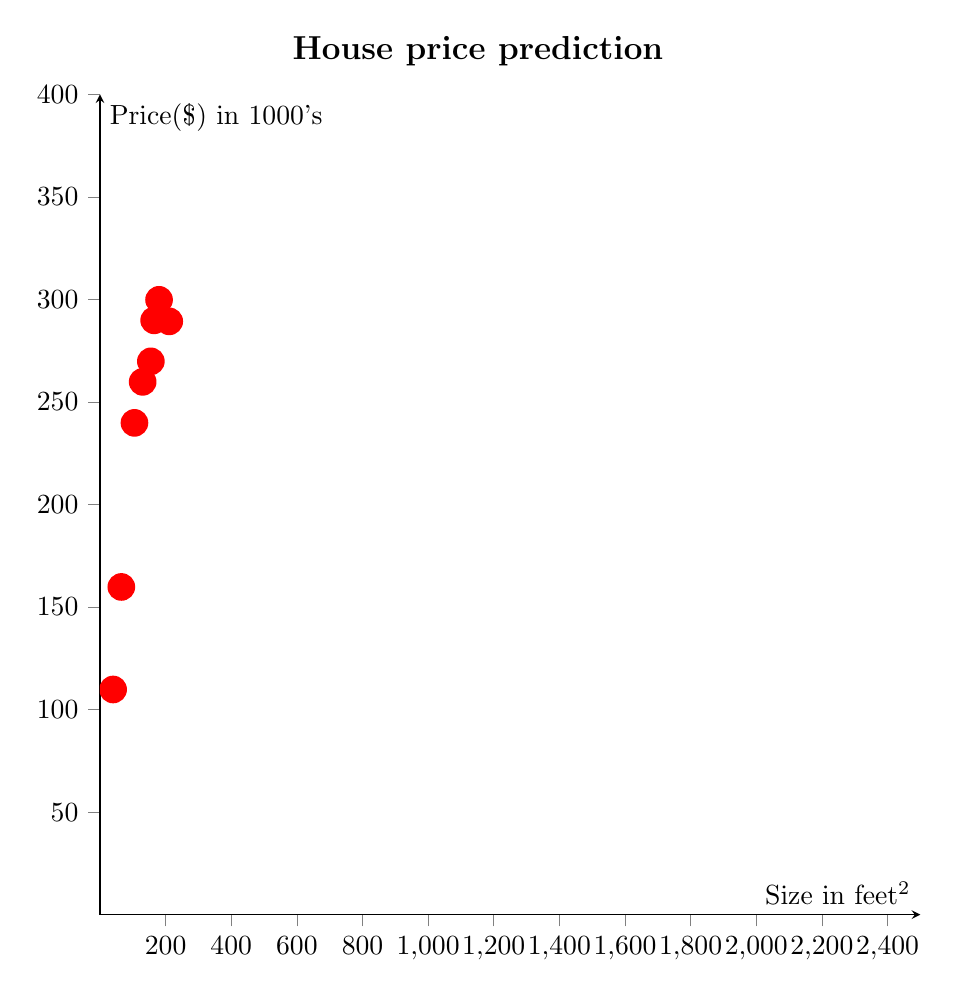
\begin{tikzpicture}
    \begin{axis}[
        axis x line=middle,
        axis y line=middle,
        width=12cm, height=12cm,     % size of the image
        grid = none,
        grid style={dashed, gray!0},
        %xmode=log,log basis x=10,
        %ymode=log,log basis y=10,
        xmin=0,     % start the diagram at this x-coordinate
        xmax= 2500,    % end   the diagram at this x-coordinate
        ymin=0,     % start the diagram at this y-coordinate
        ymax= 400,   % end   the diagram at this y-coordinate
        %/pgfplots/xtick={0,1,...,60}, % make steps of length 5
        %extra x ticks={23},
        %extra y ticks={0.507297},
        axis background/.style={fill=white},
        ylabel=Price(\$) in 1000's,
        xlabel=Size in feet$^2$,
        %xticklabels={,,},
        %yticklabels={,,},
        tick align=outside,
        tension=0.08]
      % plot the stirling-formulae
       \fill[red] (211, 289.3) circle (5pt);
       \fill[red] (180, 299.8) circle (5pt);
       \fill[red] (165, 289.8) circle (5pt);
       \fill[red] (130, 259.8) circle (5pt);
       \fill[red] (155, 269.8) circle (5pt);
       \fill[red] (105, 239.8) circle (5pt);
       \fill[red] (65, 159.8) circle (5pt);
       \fill[red] (40, 109.8) circle (5pt);
    \end{axis}
    	\node[above,font=\large\bfseries] at (current bounding box.north) {House price prediction};
\end{tikzpicture}
\\\\
Example problem: "Given this data, a friend has a house 750 square feet - how much can they be expected to get?"

\subsection*{What approaches can we use to solve this?}
\begin{itemize}
\item Straight line through data. Maybe \$150,000.
\item Second order polynomial. Maybe \$200,000.
\item One point we'll go over later is whether to use a straight or curved line.
\item Each of these techniques is a method of carrying out supervised learning.
\end{itemize}

\subsection*{We also call this a regression problem}
\begin{itemize}
\item Predict continuous valued output (price).
\item No real discrete delineation.
\end{itemize}


\begin{tikzpicture}
    \begin{axis}[
        axis x line=middle,
        axis y line=middle,
        width=12cm, height=5cm,     % size of the image
        grid = none,
        grid style={dashed, gray!0},
        %xmode=log,log basis x=10,
        %ymode=log,log basis y=10,
        xmin=0,     % start the diagram at this x-coordinate
        xmax= 1,    % end   the diagram at this x-coordinate
        ymin=-0.1,     % start the diagram at this y-coordinate
        ymax= 1.5,   % end   the diagram at this y-coordinate
        %/pgfplots/xtick={0,1,...,60}, % make steps of length 5
        %extra x ticks={23},
        extra y ticks={0, 1},
        axis background/.style={fill=white},
        ylabel=Maligant?,
        xlabel=Tumor size,
        xticklabels={,,},
        yticklabels={,,},
        tick align=outside,
        tension=0.08]
      % plot the stirling-formulae
       \fill[blue] (5, 10) circle (5pt);
       \fill[blue] (20, 10) circle (5pt);
       \fill[blue] (30, 10) circle (5pt);
       \fill[blue] (50, 10) circle (5pt);
       \fill[blue] (60, 10) circle (5pt);
       \fill[red] (50, 110) circle (5pt);
       \fill[red] (45, 110) circle (5pt);
       \fill[red] (65, 110) circle (5pt);
       \fill[red] (75, 110) circle (5pt);
       \fill[red] (89, 110) circle (5pt);
    \end{axis}
    	\node[above,font=\large\bfseries] at (current bounding box.north) {Define breast cancer as malignant or benign based on tumour size
};
\end{tikzpicture}

\begin{itemize}
\item Can you estimate the prognosis based on the tumor's size?
\item This is an example of a classification problem.
\item Classify data into one of two categories - malignant or not - with no in-betweens.
\item In classification problems, the output can only have a discrete number of potential values.
\end{itemize}

You may have many attributes to consider.

\subsection*{We also call this a regression problem}
\begin{itemize}
\item Predict continuous valued output (price).
\item No real discrete delineation.
\end{itemize}


\begin{tikzpicture}
    \begin{axis}[
        axis x line=middle,
        axis y line=middle,
        width=12cm, height=5cm,     % size of the image
        grid = none,
        grid style={dashed, gray!0},
        %xmode=log,log basis x=10,
        %ymode=log,log basis y=10,
        xmin=0,     % start the diagram at this x-coordinate
        xmax= 1,    % end   the diagram at this x-coordinate
        ymin=0,     % start the diagram at this y-coordinate
        ymax=1,   % end   the diagram at this y-coordinate
        %/pgfplots/xtick={0,1,...,60}, % make steps of length 5
        %extra x ticks={23},
        %extra y ticks={0, 1},
        axis background/.style={fill=white},
        ylabel=Age,
        xlabel=Tumor size,
        xticklabels={,,},
        yticklabels={,,},
        tick align=outside,
        tension=0.08]
      % plot the stirling-formulae
       \fill[blue] (5, 10) circle (5pt);
       \fill[blue] (20, 10) circle (5pt);
       \fill[blue] (30, 10) circle (5pt);
       \fill[blue] (40, 10) circle (5pt);
       \fill[blue] (45, 10) circle (5pt);
       \fill[blue] (10, 30) circle (5pt);
       \fill[blue] (25, 30) circle (5pt);
       \fill[blue] (35, 30) circle (5pt);
       \fill[blue] (15, 70) circle (5pt);
       \fill[blue] (25, 60) circle (5pt);
       \fill[blue] (15, 50) circle (5pt);
       \fill[blue] (20, 50) circle (5pt);
       \fill[blue] (30, 50) circle (5pt);
       \fill[blue] (40, 50) circle (5pt);
       \fill[blue] (25, 60) circle (5pt);
       \fill[blue] (55, 60) circle (5pt);
       \fill[red] (50, 80) circle (5pt);
       \fill[red] (45, 80) circle (5pt);
       \fill[red] (65, 90) circle (5pt);
       \fill[red] (25, 40) circle (5pt);
       \fill[red] (55, 70) circle (5pt);
       \fill[red] (50, 90) circle (5pt);
       \fill[red] (50, 60) circle (5pt);
       \fill[red] (45, 60) circle (5pt);
       \fill[red] (65, 60) circle (5pt);
       \fill[red] (75, 20) circle (5pt);
       \fill[red] (70, 30) circle (5pt);       
       \fill[red] (30, 80) circle (5pt);
       \fill[red] (40, 70) circle (5pt);
       \fill[red] (65, 30) circle (5pt);
       \fill[red] (55, 40) circle (5pt);    
    \end{axis}
\end{tikzpicture}

\begin{itemize}
\item You can try to establish different classes based on that data by drawing a straight line between the two groups.
\item Defining the two groups with a more sophisticated function (which we'll go over later)
\item Then, when you have someone with a certain tumor size and age, you can ideally utilize that information to assign them to one of your classes.
\end{itemize}


\section*{Unsupervised learning - introduction}
\begin{itemize}
\item Second major type.
\item We use labeled datasets (as opposed to unlabeled).
\end{itemize}

\subsection*{Clustering algorithm}
\begin{itemize}
\item Google news. Groups news stories into cohesive groups.
\item Genomics.
\item Microarray data. Have a group of individuals. On each measure expression of a gene. Run algorithm to cluster individuals into types of people.
\item Organize computer clusters. Identify potential weak spots or distribute workload effectively.
\item Social network analysis. Customer data.
\item Astronomical data analysis. Algorithms give amazing results.
\end{itemize}

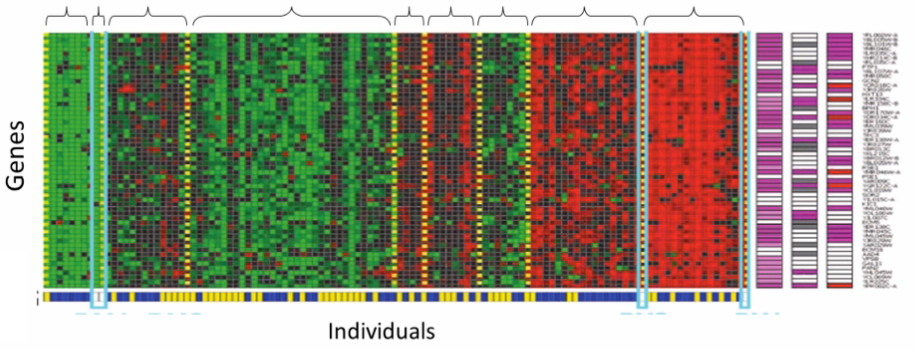
\includegraphics[width=\textwidth]{resources/genes}

\subsection*{Cocktail party problem}

\begin{itemize}
\item Depending on where your microphone is, record slightly different versions of the conversation.
\item Give the recordings to the algorithm.
\item It is discovered that there are two audio sources.
\end{itemize}

$$[W,s,v] = svd((repmat(sum(x.*x,1), size(x,1),1).*x)*x');$$

\end{document}